\subsection{Introduction}

In the mid-19th century, \cite{croll67a} and \cite{croll67b} proposed an
astronomical theory linking the Pleistocene\footnote{2 Million to 10
  thousand years ago} ice ages with periodic changes in the Earth's
orbit around the Sun. Croll's ideas were later refined and elaborated
by \cite{milankovitch41}. Since this theory was put forward, much
evidence has been found to support it.

The original Milankovitch theory identifies three types of orbital
variations which could act as climate forcing mechanisms, obliquity of
the Earth's axis, eccentricity of the Earth orbit around the Sun, and
precession of the equinoxes. Each variation has its specific time
period.

To allow proper representation of orbital variations for climate
simulations in ECHAM5, two orbits are given. The first one is based on
very precise orbit determination principles to reflect short term
variations for todays climate. It is using the VSOP (Variations
S\'{e}culaires des Orbites Plan\'{e}taires) analytical solution by
\cite{bretagnon88}. This analytical solution is representing the
todays orbit for an interval of -4000 and +8000 years with respect to
the epoch J2000.0 very accurate. The second orbit given is using the
basic Kepler laws only, allowing for simple adjustment for
paleoclimate studies using the long term series expansions for
obliquity, eccentricity, and precession by \cite{laskar93}.

Before starting to describe the used orbits, the three basic orbital
parameters for variations in climate are described as there are the
obliquity $i$, the eccentricity $e$, and the precession expressed as
the longitude of the perihelion $\omega$ with respect to the equinox.

\subsection{\label{obl}Obliquity}

Today the Earth is tilted on its rotational axis at an angle of 23.4\grad
relative to a perpendicular to the orbital plane of the Earth. Over a
\~ 41000 year time period, this angle of inclination fluctuates
between 22\grad and 24.5\grad, influencing the latitudinal distribution
of solar radiation.

\begin{figure}[htb]
\[
\ifpdf
\includegraphics[width=12cm]{science/obliquity.pdf}
\else
\includegraphics[width=12cm]{science/obliquity.eps}
\fi
\]
\caption{Obliquity}
\end{figure}

Obliquity does not influence the total amount of solar radiation
received by the Earth, but affects the distribution of insolation in
space and time. As obliquity increases, so does the amount of solar
radiation received at high latitudes in summer, whilst insolation
decreases in winter. Changes in obliquity have little effect at low
latitudes, since the strength of the effect decrease towards the
equator. Consequently, variations in the Earth's axial tilt affect the
strength of the latitudinal temperature gradient. Increased tilt has
the effect of raising the annual receipt of solar energy at high
latitudes, with a consequent reduction in the latitudinal temperature
gradient.

\subsection{Eccentricity}

The Earth's orbit around the Sun is not perfectly circular but follows
an elliptical path (see Figure \ref{eccentricity}). A second orbital
variation involves the strength of the ellipse, or eccentricity. This
parameter, $e$, is determined by Equation \ref{ecccalc}.

\begin{equation}
e = \frac{1}{2} \frac{(a^2 - b^2)}{a} 
\label{ecccalc}
\end{equation}

When the orbit is circular, the semimajor axis $a$ and semiminor axis
$b$ are equal and $e = 0$. The Earth's orbit has been found to vary
from being near circular ($e = 0.005$) to markedly elliptical ($e =
0.06$) with two primary periodicities of approximately 96000 and
413000 years \citep{berger76}. The current value of $e$ is 0.0167
\citep{meeus98}. Variations in eccentricity influence the total amount
of solar radiation incident at the top of the Earth's atmosphere. With
maximum eccentricity, differences in solar radiation receipt of about
30 \% may occur between perihelion and aphelion \citep{goodess92}.

\begin{figure}[htb]
\[
\ifpdf
\includegraphics[width=12cm]{science/eccentricity.pdf}
\else
\includegraphics[width=12cm]{science/eccentricity.eps}
\fi
\]
\caption{\label{eccentricity}Eccentricity}
\end{figure}

\subsection{Precession}

The third orbital variation is that of precession. The Sun lies at one
of the focal points of the Earth's orbital ellipse. Due to the
gravitational interaction of other planetary bodies in the solar
system, primarily the Moon and the planet Jupiter, the perihelion (the
point at which the Earth passes closest to the Sun) moves in space
with a consequent shifting or precessing of the elliptical orbit. This
phenomenon is known as the precession of the equinoxes, and effects
the intensity of the seasons.

\begin{figure}[htb]
\[
\ifpdf
\includegraphics[width=12cm]{science/precession.pdf}
\else
\includegraphics[width=12cm]{science/precession.eps}
\fi
\]
\caption{Precession}
\end{figure}

Precession has two components: an axial precession, in which the
torque of the other planets exerted on the Earth's equatorial bulge
causes the rotational axis to gyrate like a spinning top, and an
elliptical precession, in which the elliptical orbit of the Earth
itself rotates about one focus. The net effect describes the
precession of the equinoxes with a period of 22000 years. This term is
modulated by eccentricity which splits the precession into periods, of
19000 and 23000 years \citep{crowell91}.

Like obliquity, precession does not affect the total amount of solar
energy received by the Earth, but only its hemispheric distribution
over time. If the perihelion occurs in mid-June i.e. when the Northern
Hemisphere is tilted toward the Sun, then the receipt of summer solar
radiation in Northern Hemisphere will increase. Conversely, if the
perihelion occurs in December, the Northern Hemisphere will receive
more solar radiation in winter. It should be clear that the direction
of changes in solar radiation receipt at the Earth's surface is
opposite in each hemisphere.


\section{Precise orbit determination based on VSOP87}

\subsection{VSOP --- Variations S\'{e}culaires des Orbites Plan\'{e}taires}

From an analytical solution of the motion of the planets expressed
with elliptic elements \citep{bretagnon82} the position of planets is
expressed as a Poisson series expansion. Different sets of coordinate
representations have been derived. The solution used in ECHAM5 for the
position of Earth is based on heliocentric spherical coordinate
variables and the reference frame is the mean equinox and ecliptic of
date.

The position of Earth is given by the heliocentric latitude $L$ and
longitude $B$ and the distance from the Sun $R$.

This coordinates are given by the following Poisson series:

\begin{eqnarray}
L & = & \sum_{n=1}^6 L_n \sum_{k=1}^{k_N} a_{k_n} \cos(b_{k_n}+c_{k_n} \tau^n) \\
B & = & \sum_{n=1}^2 B_n \sum_{k=1}^{k_N} a_{k_n} \cos(b_{k_n}+c_{k_n} \tau^n) \\
R & = & \sum_{n=1}^5 R_n \sum_{k=1}^{k_N} a_{k_n} \cos(b_{k_n}+c_{k_n} \tau^n) 
\end{eqnarray}

where $\tau$ is reckoned in thousands of Julian years from epoch J2000.0

\begin{equation}
\tau = \frac{\mbox{Julian date} - 2 451 545}{365 250}
\end{equation} 

The coefficients for the Poisson series expansions are given in tables
\ref{tab:L1} till \ref{tab:R5} in appendix \ref{app:orbit_tables}.

To derive the required coordinates of the Sun with respect to Earth
the calculated heliocentric spehrical coordinates have to be
transformed to geocentric spherical coordinates.

First step is a transformation of the Sun's and Earth's position to
heliocentric rectangular coordinates with:

\begin{equation}
\vec{X}_s = f(L_s,B_s,R_s) \quad \mbox{and} \quad  \vec{X}_e= f(L_e,B_e,R_e)
\end{equation}

$\vec{X}$ are the heliocentric rectangular coordinates, $(L,B,R)$ are
the heliocentric spherical coordinates. The subscripts $s$ and $e$ are
denoting the Sun and Earth respectively. The transformation function
$f$ is given by:

\begin{eqnarray}
X & = & R \cos L \cos B \nonumber \\
Y & = & R \sin L \cos B \label{str}\\
Z & = & R \sin B        \nonumber
\end{eqnarray}

The geocentric rectangular coordinates are than given by:

\begin{equation}
\vec{x} = \vec{X}_s - \vec{X}_e
\end{equation}

$\vec{x}$ has to be transformed to geocentric spherical coordinates by
the inverse $f^{-1}$ of equation \ref{str}:

\begin{eqnarray}
l & = & \arctan \frac{y}{x}  
	  \quad \mbox{with} \quad l = l + 2 \pi 
          \quad \mbox{for}  \quad l < 0 \\ \nonumber
b & = & \arcsin \frac{z}{r} \\
r & = & \sqrt{x^2+y^2+z^2} \nonumber
\end{eqnarray}

The next step is the transformation from the ecliptic geocentric to
equatorial geocentric coordinates. This requires the obliquity (or
inclination) $i$ of Earth.  This is a slowly varying property of the
Earth's orbit, see section \ref{obl}. For the calculation of the
actual obliquity a polynomial series developed by \cite{laskar93} is
used:

\begin{eqnarray}
i & = &   84381.448     \\ \nonumber
  &   & - 4680.93 U - 1.55 U^2 + 1999.25 U^3 - 51.38 U^4  - 249.67 U^5 \\ \nonumber 
  &   & -   39.05 U^6 + 7.12 U^7 +   27.87 U^8  +  5.79 U^9  +   2.45 U^10
\end{eqnarray}

$U$ is the time given as $U = 0.01 \tau$. The transformation to
equatorial geocentric coordinates is given by:

\begin{eqnarray}
\alpha  & = & \arctan \left(\frac{\cos b \sin l \cos i 
             - \sin b \sin i}{\cos b \cos L}\right)
	      \quad \mbox{with} \quad \alpha = \alpha + 2 \pi 
              \quad \mbox{for}  \quad \alpha < 0 \\ \nonumber
\delta  & = & \arcsin \left(\sin b \cos i + \cos b \sin i \sin l\right)
\end{eqnarray} 

There is another effect which has to be considered in determining the
Sun's position in geocentric coordinates and this is the aberration.
Aberration is the angular discrepancy between the apparent position of
a star and its true position, arising from the motion of an observer
relative to the path of the beam of light observed. This motion is the
result of velocity components like the speed of the diurnal rotation
of the Earth and its orbital speed in revolving around the sun. The
change in Earth's position due to aberration regarding the Sun is
given by:

\begin{eqnarray}
\Delta \alpha & = & -9.93639\,10^{-5} 
                    \frac {\left( \cos \alpha \cos \lambda \cos i 
                   + \sin \alpha \sin \lambda\right) } {\cos \delta} \\
\Delta \delta & = & -9.93639\,10^{-5} \cos \lambda \left( \sin i \cos \delta 
                   - \sin \alpha \sin\delta \cos i\right) 
                   + \cos \alpha \sin \delta \sin \lambda
\end{eqnarray}

where $\lambda$ is the longitude and $e$ the eccentricity of the Sun
given by

\begin{equation}
\lambda = L_0 + C 
\end{equation}

where $L_0$ is the Sun's longitude of the ascending node, and $C$ the
position of the Sun, these are in terms of mean anomaly $M$ and
eccentricity $e$ (in degrees), and time $t$ in hundreds of Julian
years:

\begin{eqnarray}
L_0 & = & 280.46646 + 36000.76983 \, t + 0.0003032 \, t^2                  \\
M   & = & 357.52910 + 35999.05028 \, t - 0.0001561 \, t^2                  \\
e   & = & 0.016708617 - 0.000042040 \, t + 0.0000001236 \, t^2             \\ 
    &   & \\ \nonumber
C   & = & e \, (2-0.25 \, e^2) \sin M 
                + 1.25 \, e^2 \sin 2M 
                + 1.083 \, e^3 \sin 3M
\end{eqnarray}

with

\[
t = \frac{\mbox{Julian date} - 2451545}{36525}
\]

So, the final position is 

\begin{eqnarray}
\alpha & = & \alpha + \Delta \alpha \\
\delta & = & \delta + \Delta \delta
\end{eqnarray}

Finaly the mean sidereal time in degrees has to be determined:

\begin{eqnarray}
\theta_0 & = & \left( 280.46061837 
                + 360.98564736629 \cdot 36525 \, t 
                + 0.000387933 \, t^2 
                - \frac{t^3}{38710000}\right) \\ \nonumber
& & \quad \mbox{with} \theta_0 = \theta_0 \mbox{mod} 360
\end{eqnarray}

\subsection{Nutation}

Nutation is a small wobble of the Earth's rotational axis with an
amplitude of about 9 arcsec and period of up to 18.6 years.
Traditionally, nutation is represented by variations in ecliptic
longitude and obliquity (the angle between the ecliptic and the
equator). Current models represent the nutation quantities with
well-defined series \citep{seidelmann82}.

The nutation of the Earth is handled by the following equations and
added before the transformation from the geocentric ecliptic to the
geocentric equatorial coordinate system is performed.

Five auxilliar variables must be calculated which allows the further
expansion of a sine/cosine series for the nutation. The five variables
are

\begin{itemize}
\item longitude of the mean ascending node of the lunar orbit
      on the ecliptic, measured from the mean equinox of date
      \begin{equation}
      \Omega =   125.0445222 -   1934.1362608 \, t + 0.00207833 \, t^2 + 2.220e-6 \, t^3
      \end{equation}
\item mean longitude of the Sun minus the mean longitude of the Sun's perigee
      \begin{equation}
      M      =   357.5277233 +  35999.0503400 \, t - 0.00016030 \, t^2 - 3.330e-6 \, t^3
      \end{equation}
\item mean longitude of the Moon minus the mean longitude of the Moon's perigee
      \begin{equation}
      M'     =   134.9629814 + 477198.8673981 \, t + 0.00869720 \, t^2 + 1.778e-5 \, t^3
      \end{equation}
\item mean longitude of the Moon minus the mean longitude of the Moon's node
      \begin{equation}
      F      =    93.2719103 + 483202.0175381 \, t - 0.00368250 \, t^2 + 3.056e-6 \, t^3
      \end{equation}
\item mean elongation of the Moon from the Sun
      \begin{equation}
      D      =   297.8503631 + 445267.1114800 \, t - 0.00191420 \, t^2 + 5.278e-6 \, t^3
      \end{equation}
\end{itemize}

The table \ref{tab:nut} with the require coeeficients is given in
appendix \ref{app:orbit_tables}.

\section{Kepler based orbit for paleoclimate applications}

The three components of the orbital variations, obliquity,
eccentricity, and precession together effect both the total flux of
incoming solar radiation and also the temporal and spatial
distribution of terrestrial insolation. These variations have the
potential to influence the energy budget of the climate system
\citep{milankovitch41,berger78}, and can therefore be regarded as
possible causes of climate change over long time scales.

\cite{milankovitch41} considered the changing seasonal (precession)
and latitudinal (obliquity) patterns of incoming radiation to be
critical factors in the growth of continental ice sheets and in the
initiation of ice ages. He hypothesised that when axial tilt was small
(large latitudinal temperature gradient), eccentricity was large and
perihelion occurred during the Northern Hemisphere winter (warmer
winters and colder summers), such a configuration would allow the
persistence of accumulated snow throughout the summer months in the
Northern Hemisphere. Additionally, the warmer winters and stronger
atmospheric general circulation due to the increased temperature
gradient would increase the amount of water vapour at the high
latitudes available for snowfall.

To allow for paleoclimate studies, ECHAM5 provides an Kepler based
orbit which has as basic parameters, to be defined externally, the
long term varying orbit parameters obliquity, eccentricity, and, as
measure for the precession, the longitude of perihelion from the
equinox of date.

Used for the calculation of the position of the Sun is Lacaille's
formula which links the true anomaly $\nu$ and the eccentric anomaly
$E$:

\begin{equation}
\tan\frac{\nu}{2} = \sqrt{\frac{1+e}{1-e}}\tan\frac{E}{2}
\label{lacaille}
\end{equation} 

with $\nu = \omega$, where $\omega$ is the longitude of
perihelion. This allows the calculation of the eccentric anomaly which
is required for the Kepler equation linking the eccentric and the mean
anomaly $M$:

\begin{equation}
\label{kepler}
M = E - e \sin E
\end{equation}

First, calculate the mean anomaly $M$ of the current longitude
$\lambda$ from the true anomaly $\nu$:

\begin{equation}
M = \lambda - M(\omega) \quad \mbox{with} \quad M(\omega) = \nu - e \sin \nu  
\end{equation}

The true and mean anomaly are identical at the vernal equinox. For
solving the Kepler equation \ref{kepler} the Newton method is used:

\[
E^{m+1} = E^m - \frac{K(E^m)}{K'(E^m)} 
\]

with

\[
K(E) = M - E + e \sin E = 0 \quad \mbox{and} \quad K'(E) = 1 + e \cos E
\]

so the final iteration expression to solve is:

\begin{equation}
E^{m+1} = E^m - \frac{M - E^m + e \sin E^m}{1 + e \cos E^m}
\end{equation}
	
This iterative solver does converge for most initial values, but not
for all. This has been taken into account. For more details see
\cite{meeus98}.

The final distance between Earth and Sun is given by

\begin{equation}
R = \left(\frac{1}{1-e \cos E}\right)^2
\end{equation}

and the true anomaly $\nu$ with Lacaille's formula (equation
\ref{lacaille}).  The true longitude is $\lambda = \nu + \omega$ and
the declination of the Sun (with $i$ the obliquity (or inclination):

\begin{equation}
\delta = \sin i \sin \lambda
\end{equation}

and the right ascension:

\begin{equation}
\alpha = \tan \frac{\cos i \sin \lambda}{\cos \lambda}
\end{equation}

\section{Differences in the daily insolation due to the two given orbits}

The astronomical orbital parameters have to be transformed into the
solar constant scaled by the distance Earth --- Sun $R$ and the local
zenith angle $Z$.

For comparison of the two given orbits the difference in the orbit
parameters against the JPL DE405 are shown. The first set is for the
AMIP2 period 1978 to 1996 and the second set for 1870 till 2150.

\begin{figure}[htb]
\begin{center}
\ifpdf
\includegraphics[width=15cm]{science/dis_1978-1996.pdf}

\includegraphics[width=15cm]{science/dec_1978-1996.pdf}

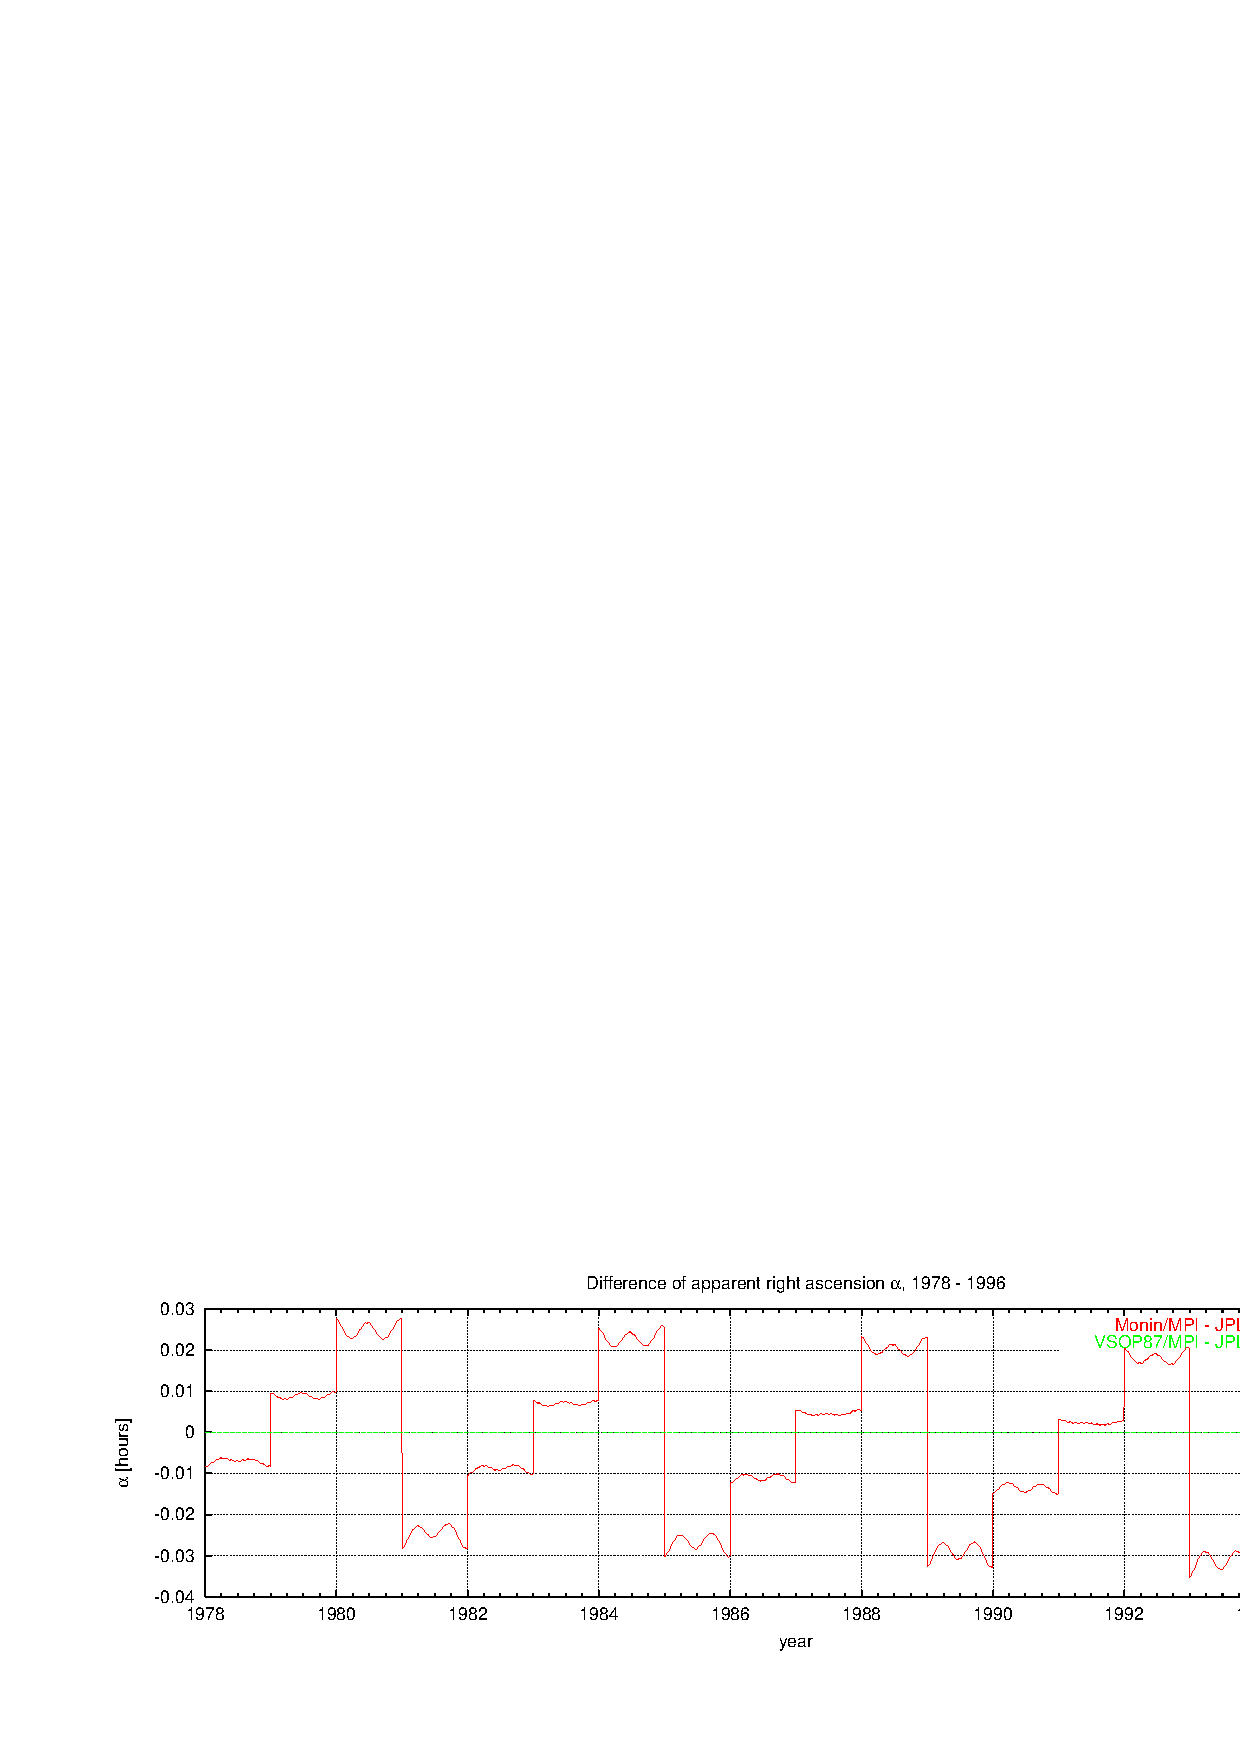
\includegraphics[width=15cm]{science/ra_1978-1996.pdf}

\includegraphics[width=15cm]{science/ga_1978-1996.pdf}
\else
\includegraphics[width=15cm]{science/dis_1978-1996.ps}

\includegraphics[width=15cm]{science/dec_1978-1996.ps}

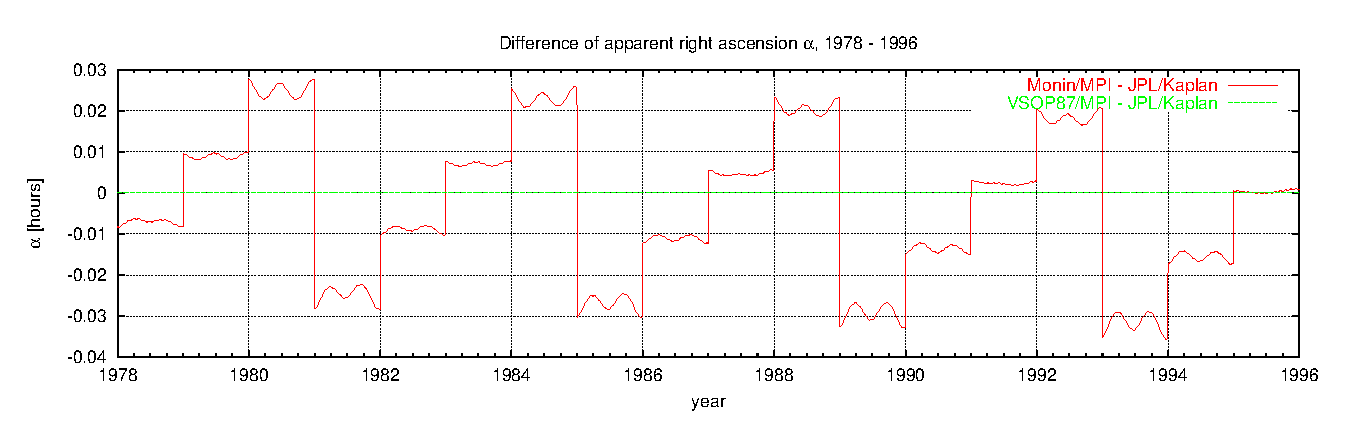
\includegraphics[width=15cm]{science/ra_1978-1996.ps}

\includegraphics[width=15cm]{science/ga_1978-1996.ps}
\fi
\end{center}
\caption{Differences between the VSOP87 and Monin orbit with respect
  to JPL's DE405 for the peride 1978 till 1996}
\end{figure}

\begin{figure}[htb]
\begin{center}
\ifpdf
\includegraphics[width=15cm]{science/dis_1870-2150.pdf}

\includegraphics[width=15cm]{science/dec_1870-2150.pdf}

\includegraphics[width=15cm]{science/ra_1870-2150.pdf}

\includegraphics[width=15cm]{science/ga_1870-2150.pdf}
\else
\includegraphics[width=15cm]{science/dis_1870-2150.ps}

\includegraphics[width=15cm]{science/dec_1870-2150.ps}

\includegraphics[width=15cm]{science/ra_1870-2150.ps}

\includegraphics[width=15cm]{science/ga_1870-2150.ps}
\fi
\end{center}
\caption{Differences between the VSOP87 and Monin orbit with respect
  to JPL's DE405 for the peride 1870 till 2150}
\end{figure}


